\section{Modello a V}
\label{modelloV}

Il Modello a V (o V-Model) è un modello di sviluppo del software. Per la precisione si tratta di un'estensione del modello a cascata. 

\begin{figure}[H]
\centering
	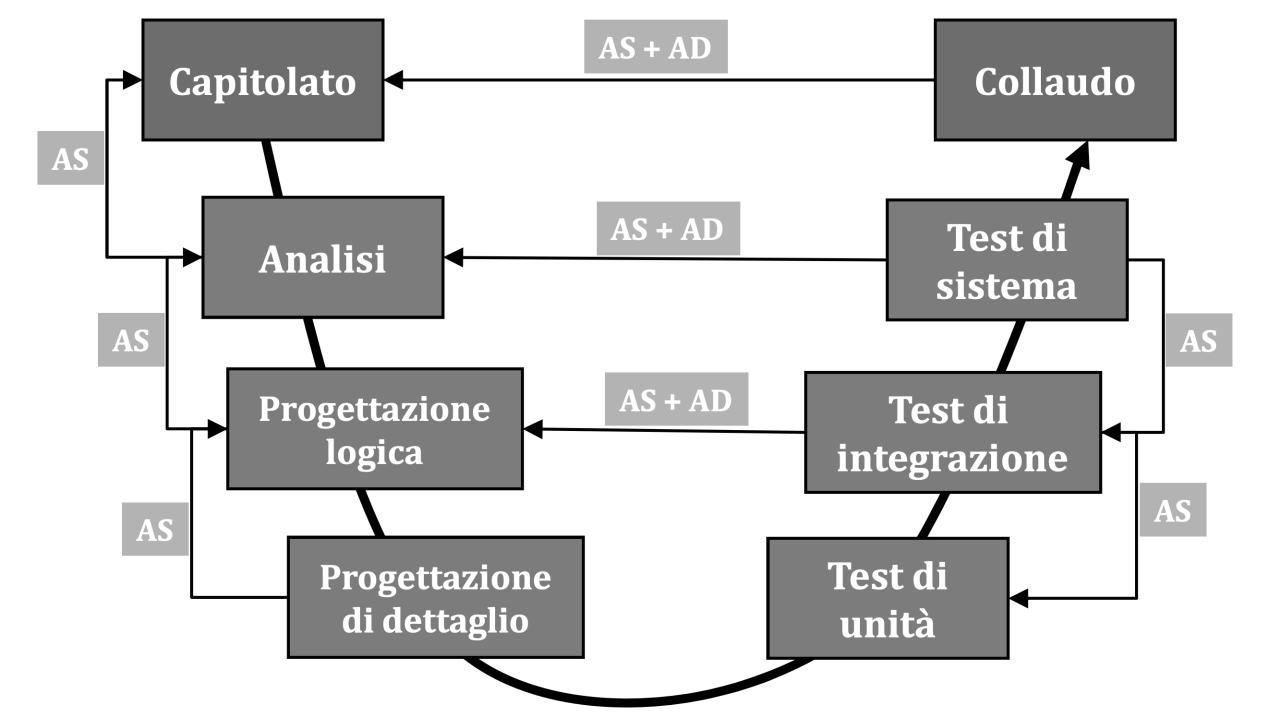
\includegraphics[width=0.7\linewidth]{./images/modellov.jpg} 
	\caption{Modello a V. Immagine dal sito web \url{https://www.math.unipd.it/~tullio/IS-1/2018/Dispense/L16.pdf}}
	\label{vmodel}
\end{figure}

Il modello a V illustra le relazioni tra ogni fase del ciclo di vita di sviluppo e la fase di testing ad essa associata. L'asse orizzontale rappresenta la completezza del progetto (da sinistra a destra); l'asse verticale il livello di astrazione (livello di astrazione minore in basso, livello di astrazione maggiore in alto).


